%!TEX root = ../these.tex

\chapter{
  Название в разработке
}
\label{ch:json}

\dots

Пример файла геометрии для простейшей раскройной карты
приведён в Листинге~\ref{lst:json-dbs}.

\lstinputlisting[
    language=Java,
    basicstyle=\footnotesize,
    showstringspaces=false,
    numbers=left,
    label={lst:json-dbs},
    captionpos=b,
    caption=JSON-файл с геометрией простейшей раскройной карты
    ]
    {media/nesting.json}

Листинг~\ref{lst:json-svg}
показывает пример простейшего SVG-файла,
сгенерированного для раскройной карты,
представленной на Листинге~\ref{lst:json-dbs}.

\lstinputlisting[
  language=XML,
  basicstyle=\footnotesize,
  showstringspaces=false,
  numbers=left,
  label={lst:json-svg},
  captionpos=b,
  caption=SVG-файл для визуализации раскроя из Листинга~\ref{lst:json-dbs}
  ]
  {media/nesting.svg}

Один из вариантов оформления
SVG-файла из Листинга~\ref{lst:json-svg}
приведён на рис.~\ref{fig:json-nesting}.
Пользовательский интерфейс
(масштабирование и прокрутка)
обеспечивается при помощи подключения
библиотеки с открытым кодом
svg-pan-zoom~\cite{bi:svg-pan-zoom}.

\begin{figure}[b]
  \centering
  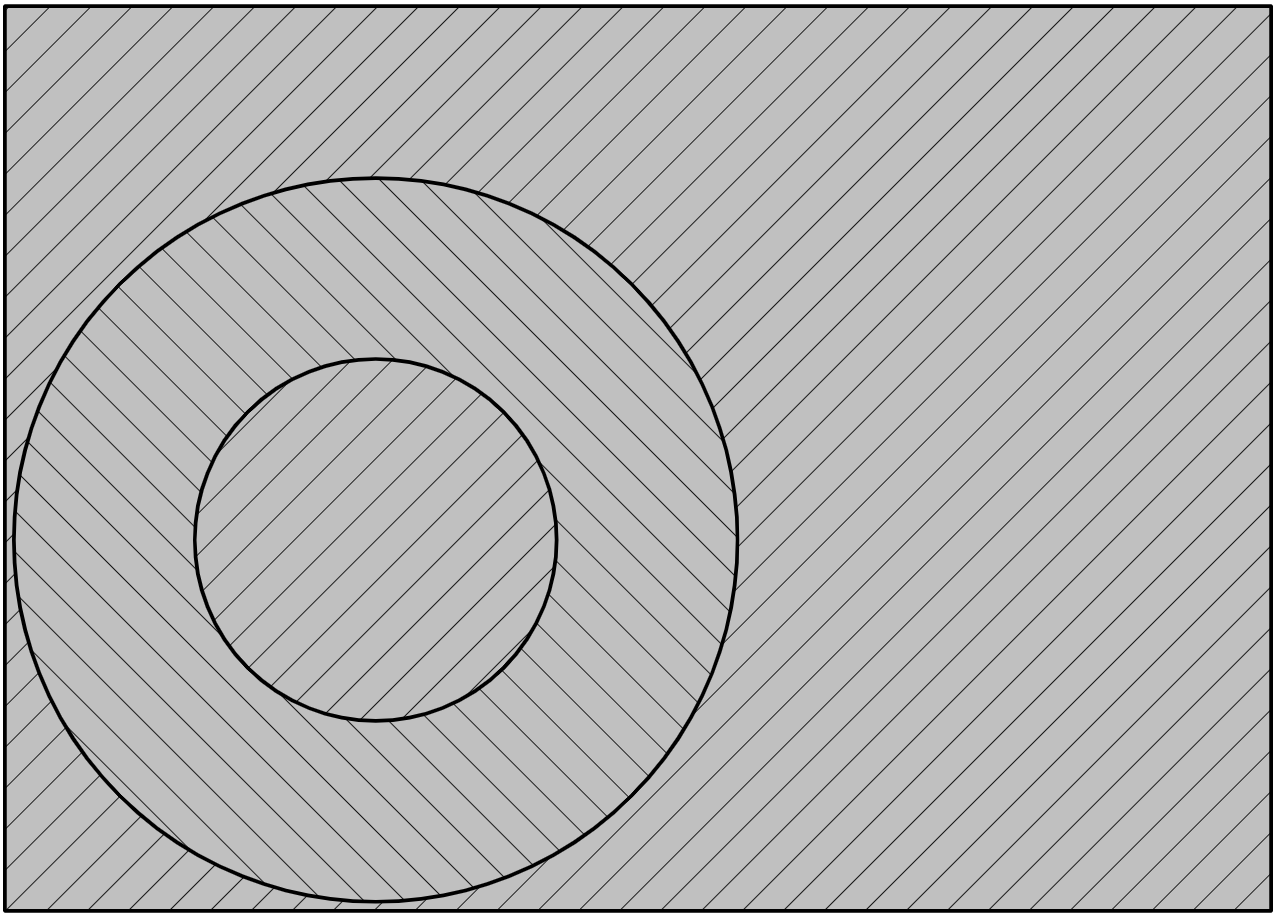
\includegraphics[width=0.5\textwidth]{nesting.png}
  \caption{Визуализация раскроя из Листинга~\ref{lst:json-dbs}}
  \label{fig:json-nesting}
\end{figure}

Для визуализации решения задачи PCGTSP
(на основе комбинации информации,
полученной из нескольких источников),
была разработана специализированная утилита
\cite{bi:j2pcgtsp},
первоначально в форме утилиты командной строки
но позднее преобразованная
для удобства использования в
Single Page Application
(SPA).
Пример созданного ею изображения
приведён на рис.~\ref{fig:pcgtsp.svg},
стр.~\pageref{fig:pcgtsp.svg}.

%!TEX root = ../these.tex

\section{Выводы по Главе \ref{ch:json}}
\label{sec:json.conclude}

\begin{enumerate}
  \item
\end{enumerate}

